\documentclass[12pt,a4paper,fleqn]{article}
\usepackage[utf8]{inputenc}
\usepackage[russian]{babel}
\usepackage{amssymb, amsmath, multicol}
\usepackage{enumitem}
\usepackage{lipsum}
\usepackage{euler}
\oddsidemargin=-15.4mm
\textwidth=190mm
\headheight=-32.4mm
\textheight=277mm
\parindent=0pt
\parskip=8pt
\pagestyle{empty}
\usepackage{graphicx}
\title{\textbf{\LARGE{Исследовательская работа по теме:\\Исследование функции дифференциальными методами}}}
\author{Известный гражданин}
\date{November 2022}
\addt\captionsrussian{\def\refname{Список литературы}}\begin{document}
\maketitle
\newpage\newpage \textbf{\LARGE{Глава I. Функция}}

\begin{center}
$y = $$sin(x)$

\end{center}
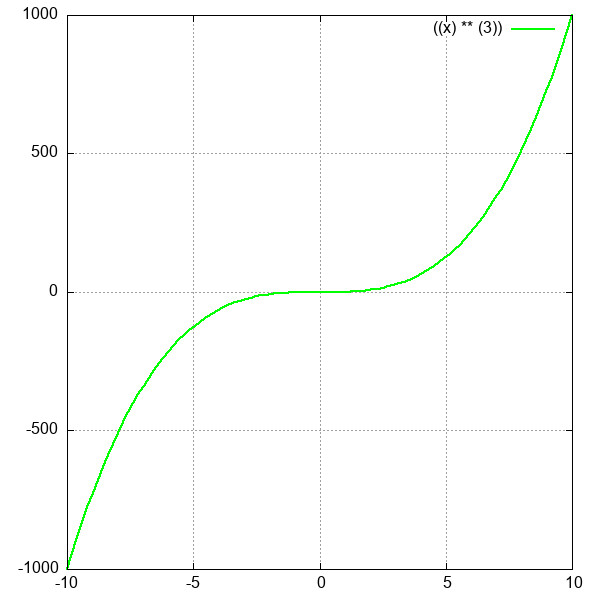
\includegraphics{GraphicDumps/plot.jpg}\newpage \textbf{\LARGE{Глава II. Визуальный анализ функции}}

Таким образом

\begin{center}
$y = $$sin(x)$

\end{center}
\newpage \textbf{\LARGE{Глава III. Дифференцирование}}

Единственное, что я не понимаю, так это то, зачем ты это читаешь

\begin{center}
 ($x)'
  = 1$\end{center}
Я придумал поистине удивительное доказательство этого факта, но поля этой книги слишком малы\ldots

\begin{center}
 ($sin(x))'
  = (1 \cdot cos(x))$\end{center}
\newpage \textbf{\LARGE{Глава IV.Упрощение выражения}}

Дураку понятно, что

\begin{center}
$(1 \cdot cos(x)) = cos(x)$\end{center}
\newpage \textbf{\LARGE{Глава V. Полученая производная}}

$y = $$sin(x)$

$y' = $$cos(x)$

\includegraphics{GraphicDumps/plot_1.jpg}\newpage \textbf{\LARGE{Глава VI. Разложение функции по формуле Тейлора}}

Глава в процессе разработки
Автору приснилось, что следующее преобразование верно

\begin{center}
\begin{center}$sin(0) = 0$\end{center}
Руководствуясь базовой логикой, получаем

\begin{center}
 ($x)'
  = 1$\end{center}
Функция производной не стоит\cite{link2}

\begin{center}
 ($sin(x))'
  = (1 \cdot cos(x))$\end{center}
Нам не объяснили на семинаре как это делать, поэтому примем на веру

\begin{center}
$(1 \cdot cos(x)) = cos(x)$\end{center}
Паршивая функция всё доказательство портит\cite{link2}

\begin{center}
\begin{center}$cos(0) = 1$\end{center}
Дураку понятно, что

\begin{center}
\begin{center}$\frac{1}{1} = 1$\end{center}
Имеем

\begin{center}
$(x-0) = x$\end{center}
Нам не объяснили на семинаре как это делать, поэтому примем на веру

\begin{center}
$x^{1} = x$\end{center}
Без комментариев\cite{link4}

\begin{center}
$(1 \cdot x) = x$\end{center}
Ребята не стоит разбираться в этом переходе. Вы молодые, шутливые, вам все легко. Это не то. Это не Чикатило и даже не архивы спецслужб. Сюда лучше не лезть. Серьезно, любой из вас будет жалеть. Лучше закройте тему и забудьте что тут писалось. Я вполне понимаю что данным сообщением вызову дополнительный интерес, но хочу сразу предостеречь пытливых - стоп. Остальных просто не найдут.

\begin{center}
 ($x)'
  = 1$\end{center}
Продвинутый читатель уже заметил, что

\begin{center}
 ($cos(x))'
  = (1 \cdot (0-sin(x)))$\end{center}
\\ title{не сложно заметить} 

\begin{center}
$(1 \cdot (0-sin(x))) = (0-sin(x))$\end{center}
Ну ты же всё равно не будешь это проверять

\begin{center}
\begin{center}$sin(0) = 0$\end{center}
Если посмотреть на выражение под другим углом, можно получить

\begin{center}
\begin{center}$(0-0) = 0$\end{center}
Отметим, что

\begin{center}
\begin{center}$\frac{0}{2} = 0$\end{center}
Segmentation fault (core dumped)

\begin{center}
$(x-0) = x$\end{center}
Продвинутый читатель уже заметил, что

\begin{center}
$(0 \cdot x^{2}) = 0$\end{center}
Британские учёные доказали, что для поддержания мозга в тонусе необходимо ежедневно дифференцировать. Продолжим наше приобщение к здоровому образу жизниn

\begin{center}
 ($0)'
  = 0$\end{center}
Обоснование этого перехода было забанено редактурой

\begin{center}
 ($x)'
  = 1$\end{center}
Ты же продолжаешь читать, да?

\begin{center}
 ($sin(x))'
  = (1 \cdot cos(x))$\end{center}
Производная дураков любит\cite{link2}

\begin{center}
 ($(0-sin(x)))'
  = (0-(1 \cdot cos(x)))$\end{center}
Для любого эпсилон больше нулю очевидно, что

\begin{center}
$(1 \cdot cos(x)) = cos(x)$\end{center}
Ну ты же всё равно не будешь это проверять

\begin{center}
\begin{center}$cos(0) = 1$\end{center}
Британские учёные доказали, что для поддержания мозга в тонусе необходимо ежедневно дифференцировать. Продолжим наше приобщение к здоровому образу жизниn

\begin{center}
\begin{center}$(0-1) = -1$\end{center}
Поэтому

\begin{center}
\begin{center}$\frac{-1}{6} = -0.166667$\end{center}
Руководствуясь базовой логикой, получаем

\begin{center}
$(x-0) = x$\end{center}
От коробки до нк все знают, что

\begin{center}
 ($0)'
  = 0$\end{center}
Я придумал поистине удивительное доказательство этого факта, но поля этой книги слишком малы\ldots

\begin{center}
 ($x)'
  = 1$\end{center}
Как было показано ранее

\begin{center}
 ($cos(x))'
  = (1 \cdot (0-sin(x)))$\end{center}
Не так страшна производная, как её находят\cite{link2}

\begin{center}
 ($(0-cos(x)))'
  = (0-(1 \cdot (0-sin(x))))$\end{center}
А теперь уберите детей от экранов

\begin{center}
$(1 \cdot (0-sin(x))) = (0-sin(x))$\end{center}
Нам не объяснили на семинаре как это делать, поэтому примем на веру

\begin{center}
\begin{center}$sin(0) = 0$\end{center}
Производная дураков любит\cite{link2}

\begin{center}
\begin{center}$(0-0) = 0$\end{center}
Как будет доказано в следующем семестре

\begin{center}
\begin{center}$(0-0) = 0$\end{center}
При этом

\begin{center}
\begin{center}$\frac{0}{24} = 0$\end{center}
Обоснование этого пререхода предостовляется читателю в качестве несложного упрожнения

\begin{center}
$(x-0) = x$\end{center}
Если вы понимаете данный переход, то я вам сочувствую

\begin{center}
$(0 \cdot x^{4}) = 0$\end{center}
Паршивая функция всё доказательство портит\cite{link2}

\begin{center}
 ($0)'
  = 0$\end{center}
Дифференциал Елена всего в 100 метрах от вас...

\begin{center}
 ($0)'
  = 0$\end{center}
Обоснование этого перехода было забанено редактурой

\begin{center}
 ($x)'
  = 1$\end{center}
Только 0.00001 процент умнейших людей планеты смогут понять этот переход

\begin{center}
 ($sin(x))'
  = (1 \cdot cos(x))$\end{center}
Обоснование этого пререхода предостовляется читателю в платном DLC

\begin{center}
 ($(0-sin(x)))'
  = (0-(1 \cdot cos(x)))$\end{center}
Ты же продолжаешь читать, да?

\begin{center}
 ($(0-(0-sin(x))))'
  = (0-(0-(1 \cdot cos(x))))$\end{center}
Если посмотреть на выражение под другим углом, можно получить

\begin{center}
$(1 \cdot cos(x)) = cos(x)$\end{center}
Обоснование этого перехода было забанено редактурой

\begin{center}
\begin{center}$cos(0) = 1$\end{center}
Как будет доказано в следующем семестре

\begin{center}
\begin{center}$(0-1) = -1$\end{center}
Телец в козероге, поэтому

\begin{center}
\begin{center}$(0--1) = 1$\end{center}
По теореме Эскобара

\begin{center}
\begin{center}$\frac{1}{120} = 0.00833333$\end{center}
Дифференциал Елена всего в 100 метрах от вас...

\begin{center}
$(x-0) = x$\end{center}
Так как 1=1, то\cite{link4}

\begin{center}
 ($0)'
  = 0$\end{center}
Для любого эпсилон больше нулю очевидно, что

\begin{center}
 ($0)'
  = 0$\end{center}
Доказательство данного факта предоставлено лицом или организацией исполняющей функции иностанного агента

\begin{center}
 ($x)'
  = 1$\end{center}
При этом

\begin{center}
 ($cos(x))'
  = (1 \cdot (0-sin(x)))$\end{center}
Поэтому

\begin{center}
 ($(0-cos(x)))'
  = (0-(1 \cdot (0-sin(x))))$\end{center}
Так как 1=1, то\cite{link4}

\begin{center}
 ($(0-(0-cos(x))))'
  = (0-(0-(1 \cdot (0-sin(x)))))$\end{center}
Положим

\begin{center}
$(1 \cdot (0-sin(x))) = (0-sin(x))$\end{center}
Продвинутый читатель уже заметил, что

\begin{center}
\begin{center}$sin(0) = 0$\end{center}
Поэтому

\begin{center}
\begin{center}$(0-0) = 0$\end{center}
Для любого эпсилон больше нулю очевидно, что

\begin{center}
\begin{center}$(0-0) = 0$\end{center}
Ну вот как этот матан тебе в жизни пригодится?

\begin{center}
\begin{center}$(0-0) = 0$\end{center}
Дифференциал Елена всего в 100 метрах от вас...

\begin{center}
\begin{center}$\frac{0}{720} = 0$\end{center}
Дураку понятно, что

\begin{center}
$(x-0) = x$\end{center}
Если посмотреть на выражение под другим углом, можно получить

\begin{center}
$(0 \cdot x^{6}) = 0$\end{center}
По теореме Эскобара

\begin{center}
 ($0)'
  = 0$\end{center}
Говорят

\begin{center}
 ($0)'
  = 0$\end{center}
Как было показано ранее

\begin{center}
 ($0)'
  = 0$\end{center}
Автору приснилось, что следующее преобразование верно

\begin{center}
 ($x)'
  = 1$\end{center}
Доказательство данного факта предоставлено лицом или организацией исполняющей функции иностанного агента

\begin{center}
 ($sin(x))'
  = (1 \cdot cos(x))$\end{center}
Segmentation fault (core dumped)

\begin{center}
 ($(0-sin(x)))'
  = (0-(1 \cdot cos(x)))$\end{center}
Segmentation fault (core dumped)

\begin{center}
 ($(0-(0-sin(x))))'
  = (0-(0-(1 \cdot cos(x))))$\end{center}
Паршивая функция всё доказательство портит\cite{link2}

\begin{center}
 ($(0-(0-(0-sin(x)))))'
  = (0-(0-(0-(1 \cdot cos(x)))))$\end{center}
Положим

\begin{center}
$(1 \cdot cos(x)) = cos(x)$\end{center}
Не так страшна производная, как её находят\cite{link2}

\begin{center}
\begin{center}$cos(0) = 1$\end{center}
Единственное, что я не понимаю, так это то, зачем ты это читаешь

\begin{center}
\begin{center}$(0-1) = -1$\end{center}
Руководствуясь сборником <<Задачи для подготовки к поступлению в советские ясли>>\cite{link1}

\begin{center}
\begin{center}$(0--1) = 1$\end{center}
Если вы не понимаете этот переход, то я вам сочувствую

\begin{center}
\begin{center}$(0-1) = -1$\end{center}
Единственное, что я не понимаю, так это то, зачем ты это читаешь

\begin{center}
\begin{center}$\frac{-1}{5040} = -0.000198413$\end{center}
[Данные удалены]

\begin{center}
$(x-0) = x$\end{center}
Нам не объяснили на семинаре как это делать, поэтому примем на веру

\begin{center}
 ($0)'
  = 0$\end{center}
Ну вот как этот матан тебе в жизни пригодится?

\begin{center}
 ($0)'
  = 0$\end{center}
//TODO: Лёша, придумай переход. У меня идеи закончились

\begin{center}
 ($0)'
  = 0$\end{center}
И хотя клуб любителей таких формул двумя блоками ниже, мы продолжаем

\begin{center}
 ($x)'
  = 1$\end{center}
\\ title{не сложно заметить} 

\begin{center}
 ($cos(x))'
  = (1 \cdot (0-sin(x)))$\end{center}
Обоснование этого пререхода предостовляется читателю в платном DLC

\begin{center}
 ($(0-cos(x)))'
  = (0-(1 \cdot (0-sin(x))))$\end{center}
В ближайшее время ожидаются осадки из ваших слёз от попыток понять этот переход

\begin{center}
 ($(0-(0-cos(x))))'
  = (0-(0-(1 \cdot (0-sin(x)))))$\end{center}
Функция производной не стоит\cite{link2}

\begin{center}
 ($(0-(0-(0-cos(x)))))'
  = (0-(0-(0-(1 \cdot (0-sin(x))))))$\end{center}
Оказывается

\begin{center}
$(1 \cdot (0-sin(x))) = (0-sin(x))$\end{center}
Ты же продолжаешь читать, да?

\begin{center}
\begin{center}$sin(0) = 0$\end{center}
Если посмотреть на выражение под другим углом, можно получить

\begin{center}
\begin{center}$(0-0) = 0$\end{center}
Как было показано ранее

\begin{center}
\begin{center}$(0-0) = 0$\end{center}
Segmentation fault (core dumped)

\begin{center}
\begin{center}$(0-0) = 0$\end{center}
//TODO: Лёша, придумай переход. У меня идеи закончились

\begin{center}
\begin{center}$(0-0) = 0$\end{center}
ИИИИЕЕЕЕсли\cite{link3}

\begin{center}
\begin{center}$\frac{0}{40320} = 0$\end{center}
Ну ты же всё равно не будешь это проверять

\begin{center}
$(x-0) = x$\end{center}
Производная дураков любит\cite{link2}

\begin{center}
$(0 \cdot x^{8}) = 0$\end{center}
Доказательство данного факта предоставлено лицом или организацией исполняющей функции иностанного агента

\begin{center}
 ($0)'
  = 0$\end{center}
Диффиринциал от производной не далеко падает\cite{link2}

\begin{center}
 ($0)'
  = 0$\end{center}
Первая производная комом\cite{link2}

\begin{center}
 ($0)'
  = 0$\end{center}
Автору приснилось, что следующее преобразование верно

\begin{center}
 ($0)'
  = 0$\end{center}
Я придумал поистине удивительное доказательство этого факта, но поля этой книги слишком малы\ldots

\begin{center}
 ($x)'
  = 1$\end{center}
Не трудно заметить

\begin{center}
 ($sin(x))'
  = (1 \cdot cos(x))$\end{center}
Британские учёные доказали, что для поддержания мозга в тонусе необходимо ежедневно дифференцировать. Продолжим наше приобщение к здоровому образу жизниn

\begin{center}
 ($(0-sin(x)))'
  = (0-(1 \cdot cos(x)))$\end{center}
Британские учёные доказали, что для поддержания мозга в тонусе необходимо ежедневно дифференцировать. Продолжим наше приобщение к здоровому образу жизниn

\begin{center}
 ($(0-(0-sin(x))))'
  = (0-(0-(1 \cdot cos(x))))$\end{center}
Для любого эпсилон больше нулю очевидно, что

\begin{center}
 ($(0-(0-(0-sin(x)))))'
  = (0-(0-(0-(1 \cdot cos(x)))))$\end{center}
По теореме Эскобара

\begin{center}
 ($(0-(0-(0-(0-sin(x))))))'
  = (0-(0-(0-(0-(1 \cdot cos(x))))))$\end{center}
Диффиринциал от производной не далеко падает\cite{link2}

\begin{center}
$(1 \cdot cos(x)) = cos(x)$\end{center}
Как будет доказано в следующем семестре

\begin{center}
\begin{center}$cos(0) = 1$\end{center}
Используя выводы из теоремы 1000-7 получаем

\begin{center}
\begin{center}$(0-1) = -1$\end{center}
Единственное, что я не понимаю, так это то, зачем ты это читаешь

\begin{center}
\begin{center}$(0--1) = 1$\end{center}
Хорошо там, где производной нет\cite{link2}

\begin{center}
\begin{center}$(0-1) = -1$\end{center}
Если вы понимаете данный переход, то я вам сочувствую

\begin{center}
\begin{center}$(0--1) = 1$\end{center}
Для любого эпсилон больше нулю очевидно, что

\begin{center}
\begin{center}$\frac{1}{362880} = 2.75573e-006$\end{center}
Имеем

\begin{center}
$(x-0) = x$\end{center}
Как будет доказано в следующем семестре

\begin{center}
$(0+(2.75573e-006 \cdot x^{9})) = (2.75573e-006 \cdot x^{9})$\end{center}
Британские учёные доказали, что для поддержания мозга в тонусе необходимо ежедневно дифференцировать. Продолжим наше приобщение к здоровому образу жизниn

\begin{center}
$(0+((-0.000198413 \cdot x^{7})+(2.75573e-006 \cdot x^{9}))) = ((-0.000198413 \cdot x^{7})+(2.75573e-006 \cdot x^{9}))$\end{center}
Откуда

\begin{center}
A = $((0.00833333 \cdot x^{5})+((-0.000198413 \cdot x^{7})+(2.75573e-006 \cdot x^{9})))$\end{center}
\begin{center}
$(0+A) = ((0.00833333 \cdot x^{5})+((-0.000198413 \cdot x^{7})+(2.75573e-006 \cdot x^{9})))$\end{center}
Имеем

\begin{center}
A = $((0.00833333 \cdot x^{5})+((-0.000198413 \cdot x^{7})+(2.75573e-006 \cdot x^{9})))$\end{center}
\begin{center}
$(0+((-0.166667 \cdot x^{3})+A)) = ((-0.166667 \cdot x^{3})+A)$\end{center}
Таким образом

\begin{center}
A = $((0.00833333 \cdot x^{5})+((-0.000198413 \cdot x^{7})+(2.75573e-006 \cdot x^{9})))$\end{center}
\begin{center}
$(0+(x+((-0.166667 \cdot x^{3})+A))) = (x+((-0.166667 \cdot x^{3})+A))$\end{center}
\begin{center}
$y = $$(x+((-0.166667 \cdot x^{3})+((0.00833333 \cdot x^{5})+((-0.000198413 \cdot x^{7})+(2.75573e-006 \cdot x^{9})))))$$ + o(x^{9})$
\end{center}
\newpage\begin{thebibliography}{}
\bibitem{link1}  "A Synopsis of Elementary Results in Pure and Applied Mathematics"
\bibitem{link2}  "Сборник пословиц и поговорок кафедры высшей математики"
\bibitem{link3}  "Полное собрание лучших высказываний преподавателей МФТИ"
\bibitem{link4}  "Словарь фраз не несущих смысловой нагрузки кафедры философии. 17 издание"
\end{thebibliography}\end{document}